%% abtex2-modelo-trabalho-academico.tex, v-1.9.2 laurocesar
%% Copyright 2012-2014 by abnTeX2 group at http://abntex2.googlecode.com/ 
%%
%% This work may be distributed and/or modified under the
%% conditions of the LaTeX Project Public License, either version 1.3
%% of this license or (at your option) any later version.
%% The latest version of this license is in
%%   http://www.latex-project.org/lppl.txt
%% and version 1.3 or later is part of all distributions of LaTeX
%% version 2005/12/01 or later.
%%
%% This work has the LPPL maintenance status `maintained'.
%% 
%% The Current Maintainer of this work is the abnTeX2 team, led
%% by Lauro César Araujo. Further information are available on 
%% http://abntex2.googlecode.com/
%%
%% This work consists of the files abntex2-modelo-trabalho-academico.tex,
%% abntex2-modelo-include-comandos and abntex2-modelo-references.bib
%%

% ------------------------------------------------------------------------
% ------------------------------------------------------------------------
% abnTeX2: Modelo de Trabalho Academico (tese de doutorado, dissertacao de
% mestrado e trabalhos monograficos em geral) em conformidade com 
% ABNT NBR 14724:2011: Informacao e documentacao - Trabalhos academicos -
% Apresentacao
% ------------------------------------------------------------------------
% ------------------------------------------------------------------------

%-------------------------------------------------------------------------
% Modelo adaptado especificamente para o contexto do PPgSI-EACH-USP por 
% Marcelo Fantinato, com auxílio dos Professores Norton T. Roman, Helton
% H. Bíscaro e Sarajane M. Peres, em 2015, com muitos agradecimentos aos 
% criadores da classe e do modelo base.
%
% 20/06/2017: inclusão de "lista de quadros" com base no especificado em:
% https://github.com/abntex/abntex2/wiki/HowToCriarNovoAmbienteListing,
% de autoria de "Eduardo de Santana Medeiros Alexandre".
%
%-------------------------------------------------------------------------

\documentclass[
	% -- opções da classe memoir --
	12pt,				% tamanho da fonte
	% openright,			% capítulos começam em pág ímpar (insere página vazia caso preciso)
	oneside,			% para impressão apenas no anverso (apenas frente). Oposto a twoside
	a4paper,			% tamanho do papel. 
	% -- opções da classe abntex2 --
	%chapter=TITLE,		% títulos de capítulos convertidos em letras maiúsculas
	%section=TITLE,		% títulos de seções convertidos em letras maiúsculas
	%subsection=TITLE,	% títulos de subseções convertidos em letras maiúsculas
	%subsubsection=TITLE,% títulos de subsubseções convertidos em letras maiúsculas
	% -- opções do pacote babel --
	english,			% idioma adicional para hifenização
	%french,				% idioma adicional para hifenização
	%spanish,			% idioma adicional para hifenização
	brazil				% o último idioma é o principal do documento
	]{abntex2ppgsi}

% ---
% Pacotes básicos 
% ---
% \usepackage{lmodern}			% Usa a fonte Latin Modern			
% \usepackage[T1]{fontenc}		% Selecao de codigos de fonte.
\usepackage[utf8]{inputenc}		% Codificacao do documento (conversão automática dos acentos)
\usepackage{lastpage}			% Usado pela Ficha catalográfica
\usepackage{indentfirst}		% Indenta o primeiro parágrafo de cada seção.
\usepackage{color}				% Controle das cores
\usepackage{graphicx}			% Inclusão de gráficos
\usepackage{microtype} 			% para melhorias de justificação
\usepackage{pdfpages}     %para incluir pdf
\usepackage{algorithm}			%para ilustrações do tipo algoritmo
\usepackage{mdwlist}			%para itens com espaço padrão da abnt
\usepackage[noend]{algpseudocode}			%para ilustrações do tipo algoritmo
		
% ---
% Pacotes adicionais, usados apenas no âmbito do Modelo Canônico do abnteX2
% ---
\usepackage{lipsum}				% para geração de dummy text
% ---

% ---
% Pacotes de citações
% ---
\usepackage{hyperref}
\usepackage[brazilian,hyperpageref]{backref}	 % Paginas com as citações na bibl
\usepackage[alf,abnt-etal-list=0,abnt-etal-text=it]{abntex2cite}	% Citações padrão ABNT

% --- 
% CONFIGURAÇÕES DE PACOTES
% --- 

% ---
% Configurações do pacote backref
% Usado sem a opção hyperpageref de backref
\renewcommand{\backrefpagesname}{Citado na(s) página(s):~}
% Texto padrão antes do número das páginas
\renewcommand{\backref}{}
% Define os textos da citação
\renewcommand*{\backrefalt}[4]{
	\ifcase #1 %
		Nenhuma citação no texto.%
	\or
		Citado na página #2.%
	\else
		Citado #1 vezes nas páginas #2.%
	\fi}%
% ---

% ---
% Informações de dados para CAPA e FOLHA DE ROSTO
% ---
\instituicao{
	UNIVERSIDADE DE SÃO PAULO
	\par
	ESCOLA DE ARTES, CIÊNCIAS E HUMANIDADES
	\par
	PROGRAMA DE PÓS-GRADUAÇÃO EM SISTEMAS DE INFORMAÇÃO}

%-------------------------------------------------------------------------
% Comentário adicional do PPgSI - Informações sobre o ``título'':
%
% Em maiúscula apenas a primeira letra da sentença (do título), exceto 
% nomes próprios, geográficos, institucionais ou Programas ou Projetos ou 
% siglas, os quais podem ter letras em maiúscula também.
%
% O subtítulo do trabalho é opcional.
% Sem ponto final.
%
% Atenção: o título da Dissertação/Tese na versão corrigida não pode mudar. 
% Ele deve ser idêntico ao da versão original.
%
%-------------------------------------------------------------------------
\titulo{Estratégias de migração de máquinas virtuais para a redução da pegada de carbono na computação em nuvem verde}
\autor{\uppercase{Guilherme Fernandes Moraes da Silva}}
\local{São Paulo}

%-------------------------------------------------------------------------
% Comentário adicional do PPgSI - Informações sobre a ``data'':
%
% Colocar o ano do depósito (ou seja, o ano da entrega) da respectiva 
% versão, seja ela a versão original (para a defesa) seja ela a versão 
% corrigida (depois da aprovação na defesa). 
%
% Atenção: Se a versão original for depositada no final do ano e a versão 
% corrigida for entregue no ano seguinte, o ano precisa ser atualizado no 
% caso da versão corrigida. 
% Cuidado, pois o ano da ``capa externa'' também precisa ser atualizado 
% nesse caso.
%
% Não incluir o dia, nem o mês.
% Sem ponto final.
%-------------------------------------------------------------------------
\data{2024}
\orientador{Prof. Dr. Daniel de Angelis Cordeiro}
\tipotrabalho{Dissertação (Mestrado) / Tese (Doutorado)}

\preambulo{
Projeto de pesquisa para exame de qualificação apresentado à Escola de Artes, Ciências e Humanidades da Universidade de São Paulo como parte dos requisitos para obtenção do título de Mestre em Ciências pelo Programa de Pós-graduação em Sistemas de Informação.
\newline \newline Área de concentração: Metodologia e Técnicas da Computação
}

% ---
% Configurações de aparência do PDF final

% alterando o aspecto da cor azul
\definecolor{blue}{RGB}{41,5,195}

% informações do PDF
\makeatletter
\hypersetup{
     	%pagebackref=true,
		pdftitle={\@title}, 
		pdfauthor={\@author},
    	pdfsubject={\imprimirpreambulo},
	    pdfcreator={laTeX com abnTeX2 adaptado para o PPgSI-EACH-USP},
		pdfkeywords={abnt}{latex}{abntex}{abntex2ppgsi}{qualificação de mestrado}{dissertação de mestrado}{qualificação de doutorado}{tese de doutorado}{ppgsi}, 
		colorlinks=true,       		% false: boxed links; true: colored links
    	linkcolor=blue,          	% color of internal links
    	citecolor=blue,        		% color of links to bibliography
    	filecolor=magenta,      		% color of file links
		urlcolor=blue,
		bookmarksdepth=4
}
\makeatother
% --- 

% --- 
% Espaçamentos entre linhas e parágrafos 
% --- 

% O tamanho do parágrafo é dado por:
\setlength{\parindent}{1.25cm}

% Controle do espaçamento entre um parágrafo e outro:
\setlength{\parskip}{0cm}  % tente também \onelineskip
\renewcommand{\baselinestretch}{1.5}

% ---
% compila o indice
% ---
\makeindex
% ---

	% Controlar linhas orfas e viuvas
  \clubpenalty10000
  \widowpenalty10000
  \displaywidowpenalty10000

% ----
% Início do documento
% ----
\begin{document}

% Retira espaço extra obsoleto entre as frases.
\frenchspacing 

% ----------------------------------------------------------
% ELEMENTOS PRÉ-TEXTUAIS
% ----------------------------------------------------------
% \pretextual

% ---
% Capa
% ---
%-------------------------------------------------------------------------
% Comentário adicional do PPgSI - Informações sobre a ``capa'':
%
% Esta é a ``capa'' principal/oficial do trabalho, a ser impressa apenas 
% para os casos de encadernação simples (ou seja, em ``espiral'' com 
% plástico na frente).
% 
% Não imprimir esta ``capa'' quando houver ``capa dura'' ou ``capa brochura'' 
% em que estas mesmas informações já estão presentes nela.
%
%-------------------------------------------------------------------------
\imprimircapa
% ---

% ---
% Folha de rosto
% (o * indica que haverá a ficha bibliográfica)
% ---
\imprimirfolhaderosto*
% ---

% ---
% ---
% inserir lista de figuras
% ---
\pdfbookmark[0]{\listfigurename}{lof}
\listoffigures*
\cleardoublepage
% ---

% ---
% inserir lista de abreviaturas e siglas
% ---
%-------------------------------------------------------------------------
% Comentário adicional do PPgSI - Informações sobre ``Lista de abreviaturas 
% e siglas'': 
%
% Opcional.
% Uma vez que se deseja usar, é necessário manter padrão e consistência no
% trabalho inteiro.
% Se usar: inserir em ordem alfabética.
%
%-------------------------------------------------------------------------
\begin{siglas}
  \item[CRC] \textit{Carbon-responsive computing}
  \item[IaaS] \textit{Infrastructure as a Service}
  \item[PaaS] \textit{Platform as a Service}
  \item[SaaS] \textit{Software as a Service}
  \item[TI] Tecnologia da informação
  \item[VM] Máquina virtual
  \item[VMM] Monitor de máquina virtual
\end{siglas}
% ---


% ---
% inserir lista de símbolos
% ---
%-------------------------------------------------------------------------
% Comentário adicional do PPgSI - Informações sobre ``Lista de símbolos'': 
%
% Opcional.
% Uma vez que se deseja usar, é necessário manter padrão e consistência no
% trabalho inteiro.
% Se usar: inserir na ordem em que aparece no texto.
% 
%-------------------------------------------------------------------------
\begin{simbolos}
	\item[$ \alpha $] Letra grega minúscula Alfa
	\item[$ \beta $] Letra grega minúscula Beta
	\item[$ \gamma $] Letra grega minúscula Gama
  \end{simbolos}
  % ---

% ---
% inserir o sumario
% ---
\pdfbookmark[0]{\contentsname}{toc}
\tableofcontents*
\cleardoublepage
% ---



% ----------------------------------------------------------
% ELEMENTOS TEXTUAIS
% ----------------------------------------------------------
\textual



%-------------------------------------------------------------------------
% Comentário adicional do PPgSI - Informações sobre ``títulos de seções''
% 
% Para todos os títulos (seções, subseções, tabelas, ilustrações, etc.):
%
% Em maiúscula apenas a primeira letra da sentença (do título), exceto 
% nomes próprios, geográficos, institucionais ou Programas ou Projetos ou
% siglas, os quais podem ter letras em maiúscula também.
%
%-------------------------------------------------------------------------
\chapter{Introdução}

\section{Contextualização}

\section{Justificativa}

\section{Problema de pesquisa}

\section{Proposição de pesquisa}

\section{Objetivos}

\subsection{Objetivos gerais}

\subsection{Objetivos específicos}

\section{Método de pesquisa}

\section{Cronograma proposto}

\section{Limitações e riscos}

\section{Estrutura do documento}

\chapter{Fundamentação teórica}\label{chapter:fundamentacao-teorica}

Neste capítulo são apresentados conceitos fundamentais para o leitor entender os demais capítulos desta dissertação. Primeiro, os conceitos de máquinas virtuais e migração de máquinas virtuais são apresentados na Seção \ref{section:maquinas-virtuais}. Em seguida, a Seção \ref{section:computacao-nuvem} apresenta os conceitos de computação em nuvem e computação em nuvem verde, além de fornecer uma visão geral sobre esses temas atualmente. Por fim, a Seção \ref{section:escalonamento} introduz o conceito de escalonamento e como ele é utilizado no contexto de computação em nuvem.

\section{Máquinas Virtuais}\label{section:maquinas-virtuais}

Uma máquina virtual (VM) é um ambiente virtualizado criado pelo hipervisor, também conhecido como monitor de máquina virtual (VMM). O VMM gerencia os recursos físicos do sistema anfitrião (a máquina física) e provisiona múltiplos ambientes virtuais independentes, chamados de convidados. Sua função principal é garantir que essas VMs compartilhem os recursos físicos de forma eficiente, evitando, por exemplo, que a mesma região de memória seja alocada simultaneamente para mais de uma VM. Dessa forma, a VM atua como uma duplicata isolada e eficiente de uma máquina real, permitindo a execução de sistemas operacionais e aplicações de forma independente e segura \cite{10.1145/361011.361073}.

Entre a máquina física e as VMs, há uma camada de software que possibilita a virtualização dos recursos. Essa camada, controlada pelo VMM, permite que as VMs superem as limitações de compatibilidade de hardware e recursos, criando um ambiente mais flexível. Em sistemas tradicionais de virtualização, o VMM opera com os mais altos privilégios, enquanto as VMs funcionam com privilégios reduzidos. Isso garante que o hipervisor possa interceptar e controlar ações que, de outra forma, acessariam ou modificariam componentes críticos do hardware, assegurando o isolamento entre as VMs e a estabilidade do sistema anfitrião. Com essa separação, torna-se possível executar diversos sistemas operacionais ou aplicações simultaneamente em uma única máquina física, o que maximiza o uso dos recursos e melhora a eficiência do ambiente computacional \cite{1430629}.

A implementação de tecnologias de virtualização também relaxa as restrições impostas pelo \textit{hardware}, e amplia a flexibilidade do sistema. A virtualização oferece um ambiente abstrato e isolado para a execução de aplicações, o que permite maior escalabilidade e facilita o gerenciamento de recursos. Além disso, existe um vasto conjunto de tecnologias e conceitos que tornam essa abstração possível, proporcionando uma infraestrutura mais adaptável às demandas dinâmicas da computação moderna \cite{10.5555/2531413}.

\subsection{Migração ao vivo de Máquinas Virtuais}\label{section:migracao-ao-vivo-maquinas-virtuais}

A migração ao vivo de máquinas virtuais é um processo útil para a administração de \textit{data centers} e \textit{clusters}, pois separa o \textit{hardware} do \textit{software}, o que facilita o gerenciamento de falhas, balanceamento de carga e manutenção. Ao transferir o sistema operacional e suas aplicações como uma unidade, esse processo permite mover o estado em memória de forma eficiente e consistente, garantindo a continuidade da execução sem interrupções. Uma das principais vantagens dessa abordagem é a possibilidade de desativar a máquina original após a conclusão da migração, o que é especialmente útil para realizar a manutenção do \textit{hardware}. Ao migrar a máquina virtual completa, o processo ocorre de forma transparente para os serviços em execução, eliminando a necessidade de gerenciar detalhes internos da VM. Isso permite, por exemplo, a migração de servidores de jogos \textit{online} sem desconectar os usuários, algo inviável em métodos que dependem da reinicialização no nível da aplicação ou do redirecionamento na camada de aplicação \cite{10.5555/1251203.1251223}.

\section{Computação em nuvem}\label{section:computacao-nuvem}

A computação em nuvem surgiu como uma solução para um dos maiores desafios da indústria tecnológica: a necessidade de que usuários e empresas adquirissem e mantivessem sua própria infraestrutura para disponibilizar serviços e aplicações. Com o crescimento exponencial da \textit{internet}, a tarefa de escalar essa infraestrutura para atender à demanda crescente tornou-se cada vez mais complexa e custosa. Conforme \citeonline{4738445}, a computação em nuvem pode ser definida como um paradigma de computação distribuída em larga escala, impulsionado pelas economias de escala, no qual um conjunto de recursos --- como computação, armazenamento, plataformas e serviços --- é abstraído, virtualizado, escalonável dinamicamente e gerenciado para ser entregue sob demanda a clientes externos por meio da \textit{internet}.

Dentro desse paradigma, as plataformas de computação em nuvem geralmente oferecem serviços em três diferentes níveis: IaaS (\textit{Infrastructure as a Service}), PaaS (\textit{Platform as a Service}) e SaaS (\textit{Software as a Service}), como descrito por \citeonline{4738445}. No nível IaaS, a plataforma fornece aos usuários acesso a recursos de \textit{hardware}, como processamento e armazenamento, cobrando de acordo com a utilização. Exemplos de serviços nesse nível incluem o Amazon EC2 (\textit{Elastic Cloud Computing}) e o Amazon S3 (\textit{Simple Storage Service}). No nível PaaS, o provedor oferece um ambiente completo para desenvolvimento, teste e implantação de aplicações, exigindo que os desenvolvedores sigam um modelo de desenvolvimento predefinido, aceitando algumas restrições em troca da escalabilidade oferecida, como no caso do Azure App Service. Por fim, no nível SaaS, aplicações específicas são disponibilizadas aos usuários por meio da \textit{internet}, com a cobrança proporcional ao uso do aplicativo. Exemplos incluem o Google Drive e o YouTube.

As plataformas modernas de computação em nuvem são compostas por diversos \textit{data centers} geograficamente distribuídos ao redor do mundo. A Figura \ref{fig:microsoft-datacenters}, por exemplo, ilustra as localizações dos \textit{data centers} da Azure, da Microsoft, que somam milhões de servidores físicos \citeonline{john_roach_2021_microsoft_azure}. Essa infraestrutura geodistribuída é fundamental para atender à crescente demanda global de usuários, além de reduzir significativamente o tempo de resposta das aplicações, uma vez que a proximidade física dos servidores em relação aos usuários finais melhora a latência. A geodistribuição também oferece vantagens em termos de segurança e redundância. Se um \textit{data center} em uma determinada região ficar indisponível devido a falhas de energia, desastres naturais ou ataques cibernéticos, outro \textit{data center} em uma região distinta pode assumir temporariamente a carga computacional, assegurando a continuidade dos serviços.

\begin{figure}[htbp]
	\centering
	\caption{Localizações geográficas dos \textit{data centers} da Microsoft Azure}
		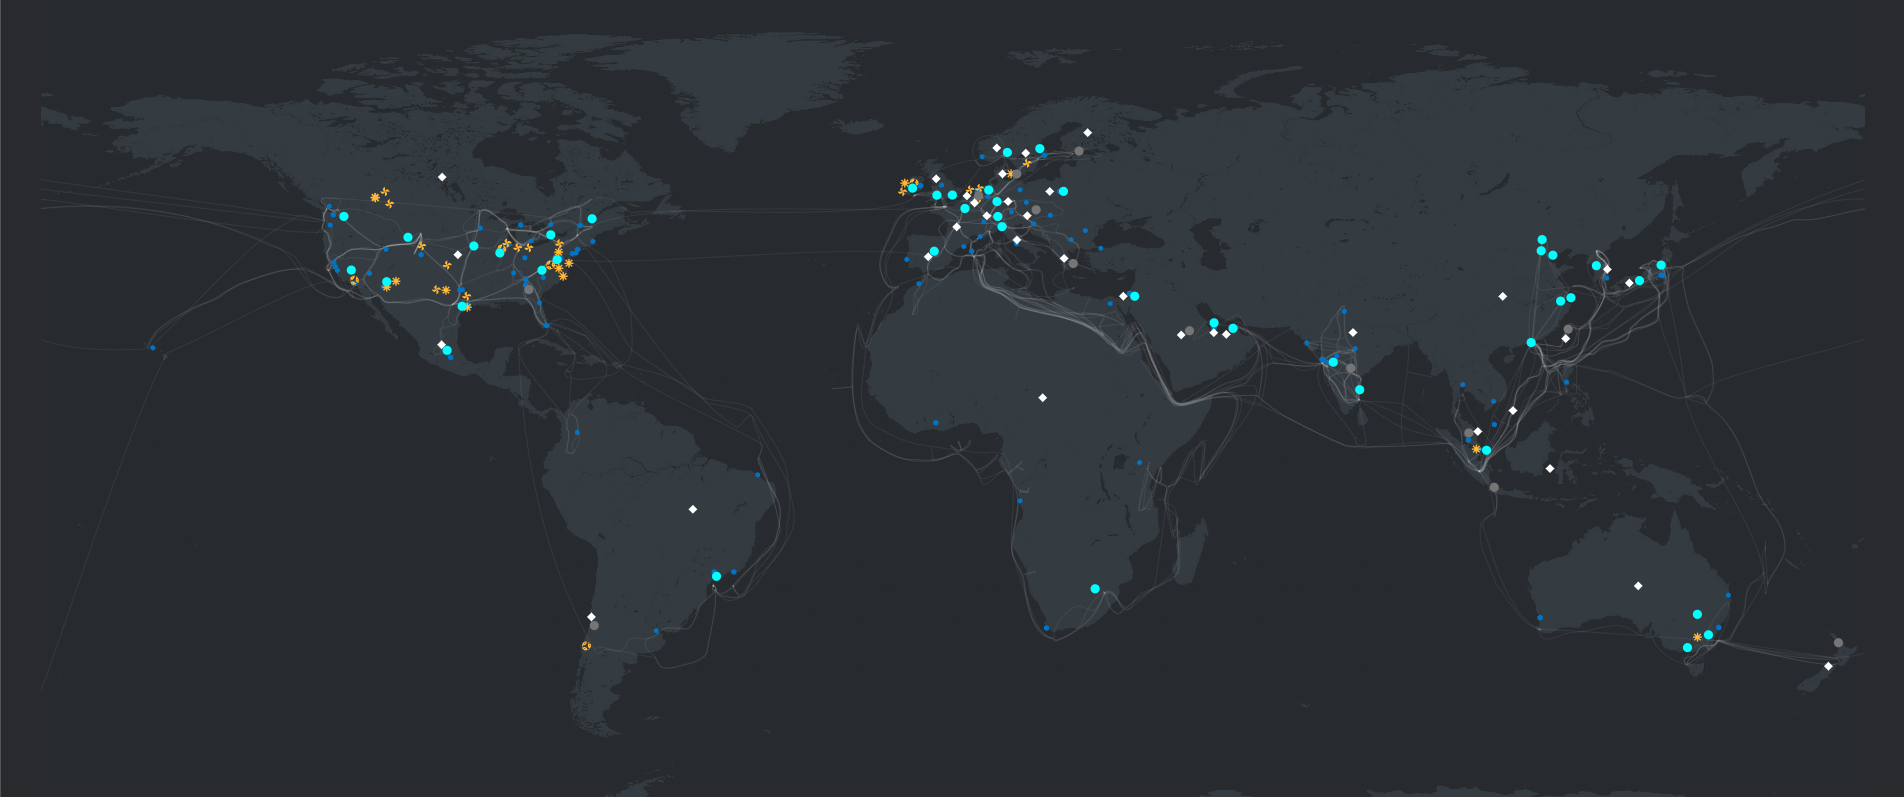
\includegraphics[width=\linewidth]{images/microsoft-datacenters.png}
	\label{fig:microsoft-datacenters}
  \source{\citeonline{azure_data_centers_locations}}
\end{figure}

\subsection{Computação em nuvem verde}

A computação verde é um paradigma que visa a criação de soluções tecnológicas ambientalmente sustentáveis e energeticamente eficientes. Esse conceito envolve o planejamento e o desenvolvimento de infraestruturas de computação e estratégias baseadas em princípios de gestão ambiental, otimização do consumo energético e práticas de reutilização. O objetivo central é promover a criação de produtos e serviços de tecnologia da informação (TI) que demandem menos energia e emitam menores quantidades de carbono. Nesse sentido, a computação verde busca reduzir o consumo de energia enquanto melhora a utilização da infraestrutura computacional, assegurando a expansão sustentável da computação em nuvem no longo prazo \cite{9793067}.

Em paralelo a esses esforços, tanto a academia quanto a indústria têm desenvolvido iniciativas para mitigar o impacto ambiental da computação em larga escala. Uma dessas iniciativas é o conceito de \textit{carbon-responsive computing} (CRC), que foca na priorização do uso de fontes de energia com menor intensidade de carbono, seja por meio de estratégias espaciais, temporais ou uma combinação de ambas. O CRC organiza-se em três estágios sequenciais, nos quais o progresso de cada fase depende da implementação adequada da anterior \cite{en14216917}.

O primeiro estágio, denominado \textit{carbon-aware computing}, compreende sistemas capazes de caracterizar e prever a intensidade de carbono, bem como medir o consumo energético associado. No segundo estágio, \textit{carbon-responsive computing}, as ações do sistema são orientadas pela intensidade de carbono em uso, ajustando o consumo energético conforme os níveis de emissões. Por fim, o terceiro estágio, \textit{carbon-resilient computing}, aborda a gestão e integração de elementos responsivos ao carbono, investigando as modificações necessárias nas infraestruturas de TI e de energia para reduzir a pegada de carbono e garantir maior resiliência ambiental \cite{en14216917}.

No contexto da infraestrutura geodistribuída da computação em nuvem, um dos principais mecanismos que permitem a implementação dessas estratégias ambientais é a migração ao vivo de máquinas virtuais, apresentada na Seção \ref{section:migracao-ao-vivo-maquinas-virtuais}. Como mencionado anteriormente, essa técnica possibilita a transferência de cargas de trabalho entre diferentes \textit{data centers} sem interrupções no serviço, promovendo o balanceamento de carga de maneira eficiente. Ao redirecionar o processamento para regiões onde a pegada de carbono é menor ou onde há disponibilidade de fontes de energia renováveis, a migração ao vivo contribui significativamente para a redução do impacto ambiental da computação em nuvem. Esse processo não só melhora a eficiência energética dos \textit{data centers}, como também apoia diretamente os objetivos de mitigação das emissões de carbono, e reforça o compromisso da computação verde com a sustentabilidade.

\section{Escalonamento}\label{section:escalonamento}

O escalonamento de tarefas é um desafio de otimização combinatória, no qual, dadas as características de um conjunto de recursos computacionais ($\alpha$) e de um conjunto de tarefas ($\beta$), o objetivo é encontrar uma alocação de recursos em tempo que minimize algum critério de otimização ($\gamma$). Essa formulação é frequentemente expressa pela notação \mbox{$\alpha$ $\vert$ $\beta$ $\vert$ $\gamma$}, introduzida por \citeonline{GRAHAM1979287}. Em ambientes de computação em nuvem, esses problemas de escalonamento ganham relevância à medida que a demanda por recursos computacionais cresce, exigindo alocações eficientes e dinâmicas que atendam a critérios como desempenho, economia de energia e sustentabilidade.

Um dos principais critérios de otimização nesse contexto é o \textit{makespan} ($C_{\max}$), que define o tempo em que a última tarefa de uma aplicação finaliza sua execução. Quando os recursos computacionais disponíveis são idênticos e conhecidos previamente, e o objetivo é minimizar o \textit{makespan} --- uma situação típica em problemas de escalonamento em \textit{clusters} --- o problema se torna fortemente NP-completo. Esse tipo de problema é denotado como $P\,\vert\,\vert\,C_{\max}$ \cite{GRAHAM1979287}.

No contexto desta dissertação, $\alpha$ representa os recursos computacionais disponíveis nos servidores dos \textit{data centers}, além de informações sobre a disponibilidade de fontes de energia com menor intensidade de carbono. Já $\beta$ descreve as exigências das VMs, como tempo de execução, prazos, memória e CPU. O critério $\gamma$ é a minimização do consumo de energia proveniente de fontes com alta intensidade de carbono, o que se alinha ao conceito de computação verde.

\chapter{Trabalhos correlatos}\label{chapter:trabalhos-correlatos}

% ----------------------------------------------------------
% ELEMENTOS PÓS-TEXTUAIS
% ----------------------------------------------------------
\postextual
% ----------------------------------------------------------

% ----------------------------------------------------------
% Referências bibliográficas
% ----------------------------------------------------------
\bibliography{referencias}

% ----------------------------------------------------------
% Glossário
% ----------------------------------------------------------
%
% Consulte o manual da classe abntex2 para orientações sobre o glossário.
%
%\glossary

% ----------------------------------------------------------
% Apêndices
% ----------------------------------------------------------

% ---
% Inicia os apêndices
% ---
\begin{apendicesenv}

% Imprime uma página indicando o início dos apêndices
%\partapendices

%-------------------------------------------------------------------------
% Comentário adicional do PPgSI - Informações sobre ``apêndice''
%
% Para todos os captions/(títulos) (de seções, subseções, tabelas, 
% ilustrações, etc.):
%     - em maiúscula apenas a primeira letra da sentença (do título), 
%       exceto nomes próprios, geográficos, institucionais ou Programas ou
%       Projetos ou siglas, os quais podem ter letras em maiúscula também.
%
% Todas  as tabelas, ilustrações (figuras, quadros, gráficos etc. ), 
% anexos, apêndices devem obrigatoriamente ser citados no texto.
%      - a citação deve vir sempre antes da primeira vez em que a tabela, 
%        ilustração etc., aparecer pela primeira vez.
%
%-------------------------------------------------------------------------
\chapter{Protocolo da revisão do estado da arte}

\chapter{Resultados da condução da revisão estado da arte}

\end{apendicesenv}
% ---


% ----------------------------------------------------------
% Anexos
% ----------------------------------------------------------

% ---
% Inicia os anexos
% ---
\begin{anexosenv}

% Imprime uma página indicando o início dos anexos
%\partanexos

\end{anexosenv}

%---------------------------------------------------------------------
% INDICE REMISSIVO
%---------------------------------------------------------------------
%%%%%MF\phantompart
%%%%%MF\printindex
%---------------------------------------------------------------------

\end{document}
